\documentclass{article}[12 pt]
\usepackage[utf8]{inputenc}
\usepackage[english]{babel}
\usepackage{tocloft}
\usepackage{lipsum}
\usepackage{sidecap}
\renewcommand\cftsecfont{\normalfont}
\renewcommand\cftsecpagefont{\normalfont}
\renewcommand{\cftsecleader}{\cftdotfill{\cftsecdotsep}}
\renewcommand\cftsecdotsep{\cftdot}
\renewcommand\cftsubsecdotsep{\cftdot}
\usepackage{graphicx}
\usepackage{hyperref,xcolor}

\definecolor{wine-stain}{rgb}{0.5,0,0}

\hypersetup
{
    colorlinks=true,
    linktoc = all,
    linkcolor = wine-stain,
    urlcolor = blue
}

\begin {document}

\title{Math Graphics README}
\author{Frank Basile, Janice Wallace, Daniel Etheridge}
\maketitle

\tableofcontents
	\section{Introduction}
		Math Graphics is the final project for Group 12. The program is a fairly robust graphing calculator capable of displaying visual representations of mathematical functions on 2D Cartesian, 2D Polar, and 3D Cartesian graphs. Aside from displaying input functions, the calculator can also display derivatives and calculate definite integrals of single-variable functions in Cartesian 2D mode. Other features of the program include the ability to output the image of the graph to a file, as well as writing the independent and dependent variable data to a data format separated by any series of ASCII characters. Other features include the ability to customize the interface through the use of color changing palettes.

	\section{Installation}
	    No specific installation instructions are required. All that is required to run the program should be an updated version of Java and the executable file named MathGraphics.jar. For the latest version of Java, please check the \href{http://www.java.com}{Java homepage}.
	    
	\section{Starting the Program}
		Math Graphics has an easy to run interface. All that is required is to double click the MathGraphics.jar executable file. 
		
	\section{How To}
		\subsection{Initial Startup}
		When the program initially starts, the grapher is in Cartesian 2D mode and the function $sin(x)$ is displayed.:
			\begin{figure}[h!]
 				\centering
 				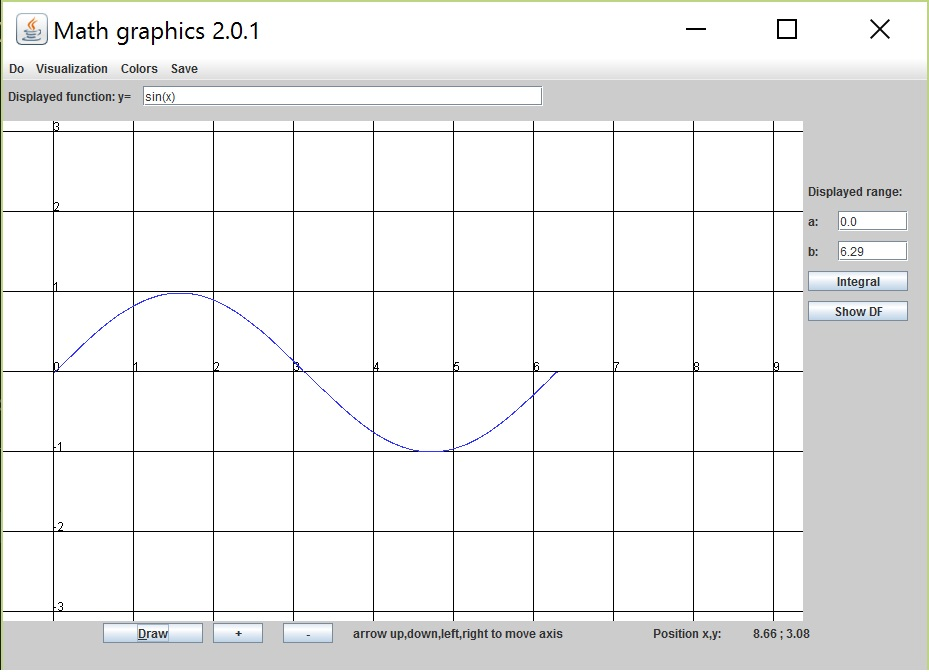
\includegraphics[scale = .90]{startupScreen}
 				\caption{The startup screen: $sin(x)$ is displayed}
 			\end{figure}
			
		\subsection{Basic 2D Navigation}
		User interactions with the Math Grapher application take place by clicking on the appropriate buttons and menu bar items. The items in the 2D Cartesian window are shown in Figure 2.  Though Polar 2D is not shown, the layout is almost identical. 
			\begin{figure}[h!] 
				\centering
				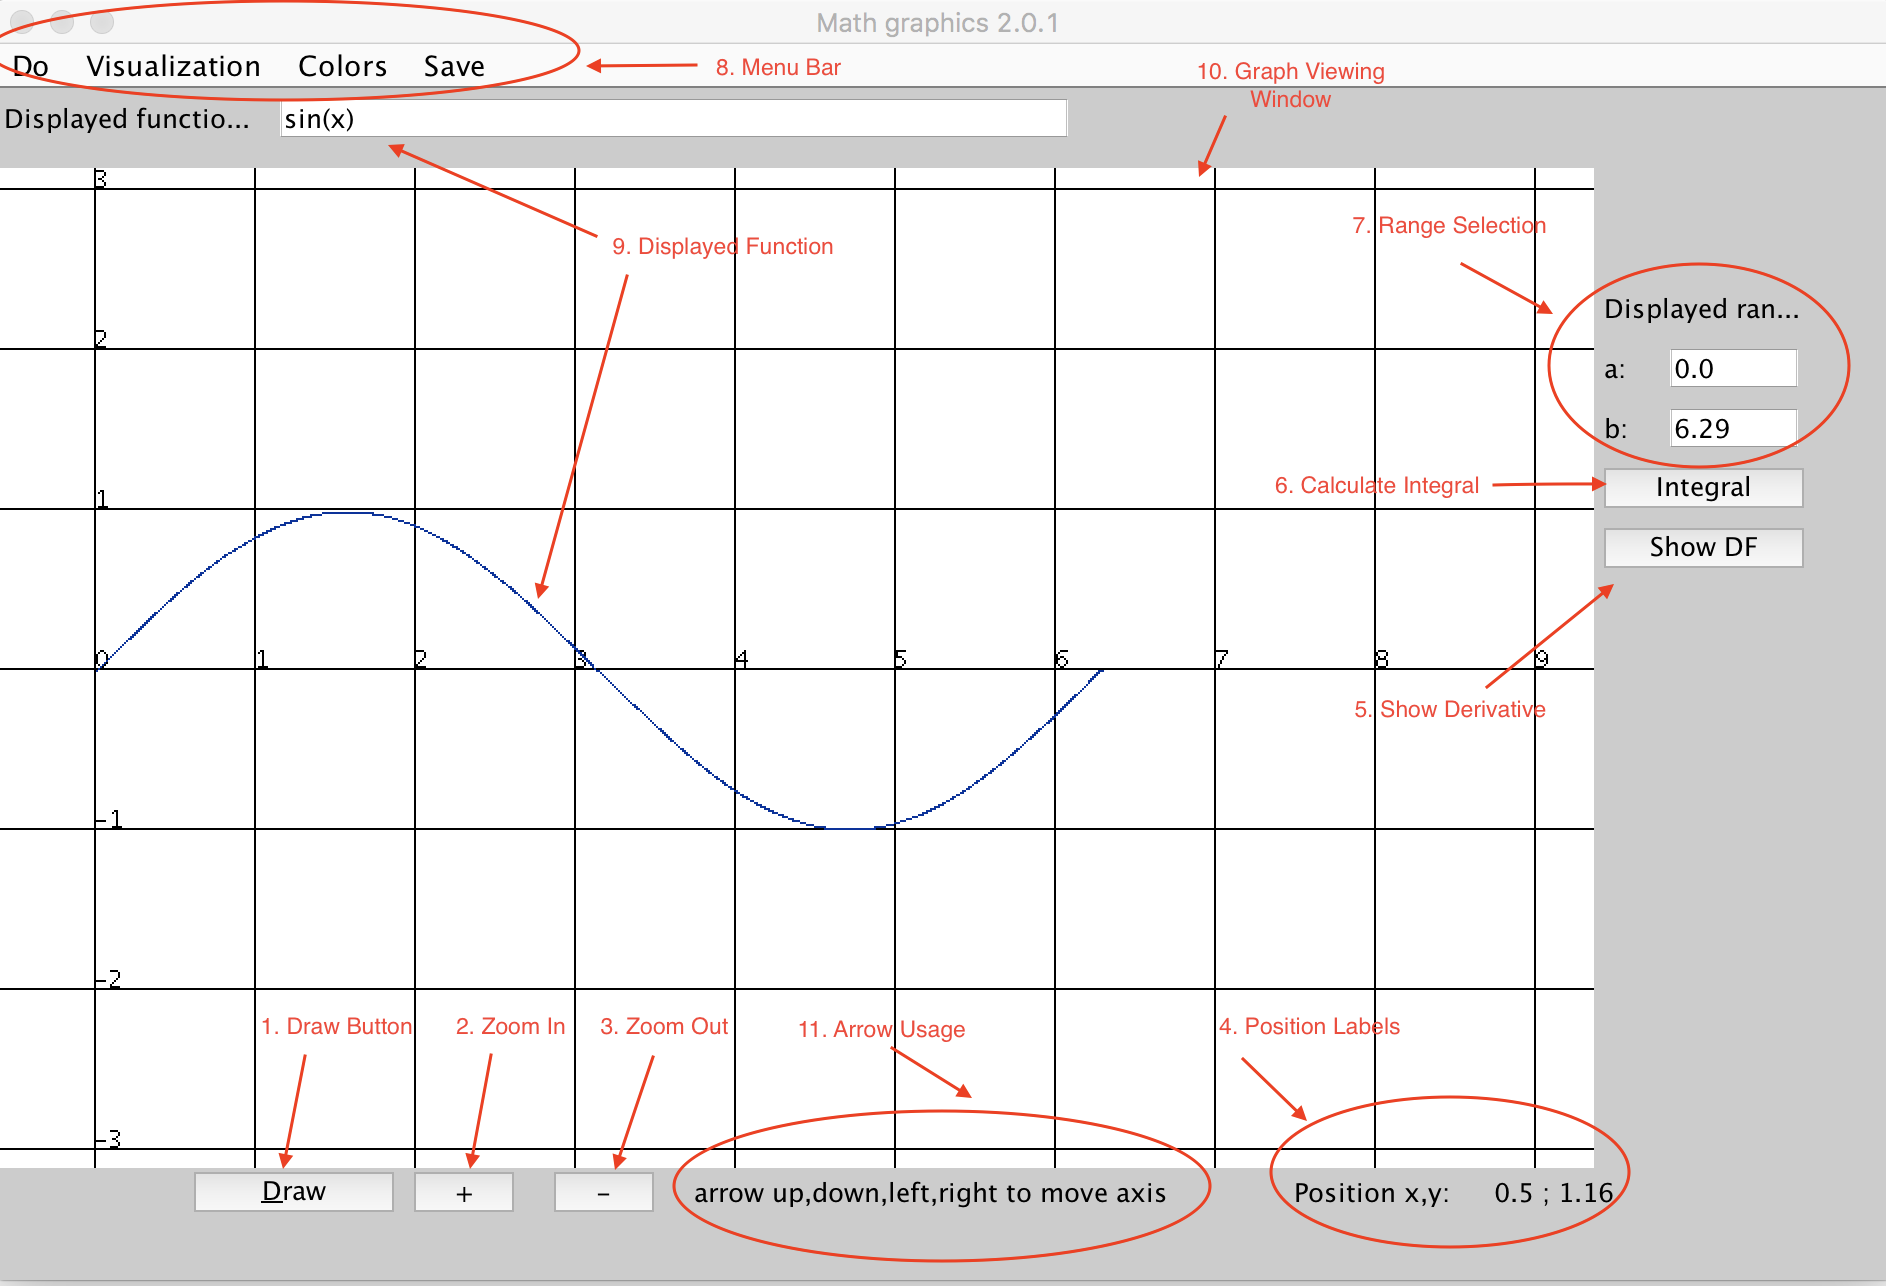
\includegraphics[scale = .40]{Map}
				\caption{Navigation items are labeled in red}
			\end{figure}
 		
			\subsubsection{Draw Button}
			The draw button (1) is used to paint the displayed function (9) into the graph viewing window (10). Any time the displayed function is changed, the draw button should be clicked. This will both validate the input and, if valid, draw the function. Alternatively, the menu bar (8) can be used by pressing ``Do" and then ``Draw" from the drop down menu.
 				
 			\subsubsection{Zoom In Function}
			The graph can be zoomed in to specific points by clicking the ``+'' button (2) located at the bottom of the screen. The graph will zoom in to the current center of the viewable graph. 
			
			\subsubsection{Zoom Out Function}
			The graph can be zoomed out of specific points by clicking the "-" button (3)  located at the bottom of the screen. The graph will zoom out from the center of the graph viewing window.
			
			\subsubsection{Position Labels}
			The position labels (4) serve as a reference point to the location on the graph viewing window (10) that the mouse pointer is currently hovering over. This can serve as an approximation to determining the input and output values of various functions.
 		
		 	\subsubsection{View the Graph of the Derivative}
 			The derivative can be displayed by pressing the ``Show DF'' button (5). Alternatively, the derivative can be displayed from the drop down menu (8) by clicking ``Do'' and ``Show DF.'' To hide the derivative simply press the ``No'' DF button (not shown). Or, from the drop down menu, select ``Do'' and ``No DF''.
 				\begin{figure}[h!]
 					\centering
 					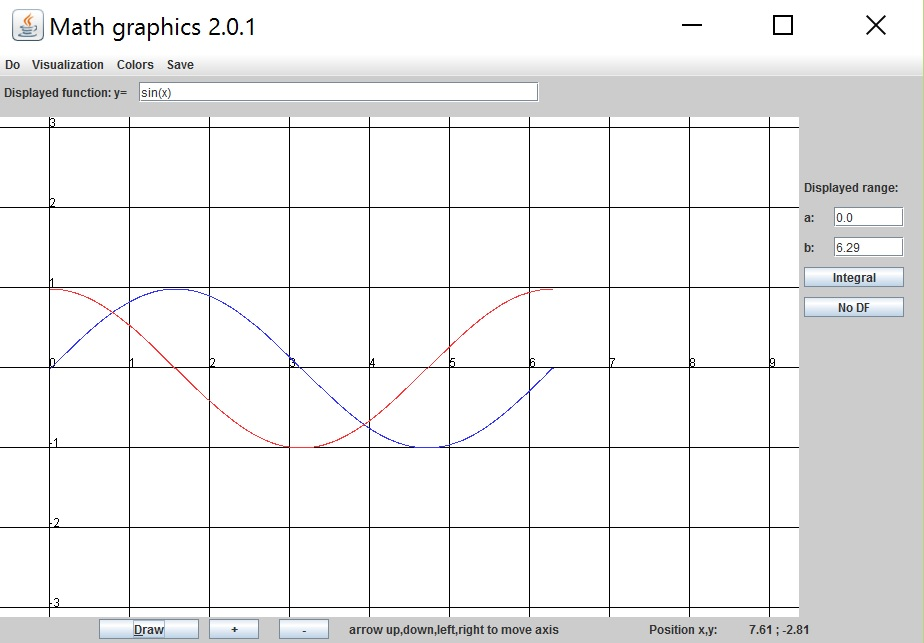
\includegraphics[scale = .85]{showDF}
					\caption{The derivative drawn after ``Show DF'' selected}
 				\end{figure}	
			
			\subsubsection{Integral Calculations}
			Definite integral calculations can be performed by pressing the ``Integral" button (6). After pressing the integral button, a new window will appear.
				\begin{figure}[h!]
					\centering
					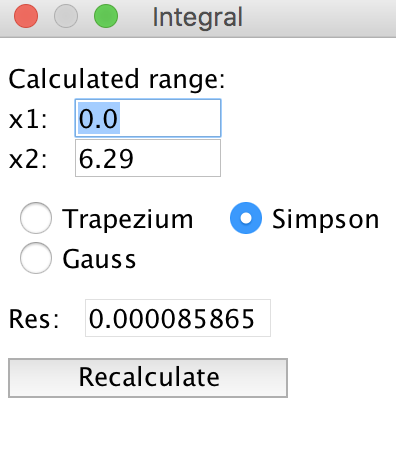
\includegraphics[scale=.5]{integral}
					\caption{Integral pop-up window}
				\end{figure}\\
				Once the integral window appears, the default range will be whatever range a and b were set to on the main display. The user has three integral calculations they can choose from: Simpson, Trapezium, and Gauss. Due to the way calculations are performed, there may be slight differences between the three - but usually no more than several thousandths. After a range is entered, and a selection made, the user will hit the recalculate button. In the result field, the newest calculation will appear.
				
			\subsubsection{Range Changes}
 			Range changes can be made to the displayed function. In order to do this, simply change the values of fields $a$ and $b$ (7). Only valid numeric values can be input to these fields. It is not a requirement that $a < b$ as both the function and derivative can be drawn with $a \leq b$ or $a \geq b$. After any changes are made, it is necessary to hit the ``Draw" button (1) or from the drop-down menu bar, select ``Do" and then ``Draw."
			
			\subsubsection{Menu Bar}
			The Menu Bar (8) provides the user with the ability to perform some of the same functions as the clickable buttons. The "Do" Menu allows the user to redraw the function, bring up the integral window, and show or hide the derivative of the displayed function. The ``Visualization" menu allows the user to view the graph in Cartesian 2D, Polar 2D or Cartesian 3D modes. The "Colors" menu gives the option for the user to change the color of the interface, and the ``Save" menu offers the opportunity to save the displayed image or export the data to a file. 
 	
			\subsubsection{Displayed Function}
			The Displayed Function field is perhaps one of the most important 
 				
\end {document}